\chapter{Evaluation}\label{chap:eval}

A user study was conducted to evaluate Replico's efficiency, effectiveness, and user-friendliness. The main goal was determining how easily users could communicate points of interest within the virtual environment using Replico. Secondary goals included assessing ease of use and overall user experience. The study aimed to answer four key research questions:

\begin{itemize}
    \item \textbf{RQ1}: How efficiently can users create a point of interest on a given object?
    \item \textbf{RQ2}: How effectively does Replico notify users when a point of interest is created?
    \item \textbf{RQ3}: How useful is the world-in-miniature metaphor for communicating points of interest? How useful is the representation of user locations on the replica for understanding intent? 
    \item \textbf{RQ4}: How user-friendly is Replico, and how much physical effort is required to use it? 
\end{itemize}

\section{Setup}

    The user study was conducted at FEUP, in the GIG laboratory in room I220. The setup included two VR-ready computers connected to a local network. One computer was equipped with an Intel Core i9-13900KF CPU, an NVIDIA GeForce RTX 4090 GPU, and 32 GB of RAM, while the other had an Intel Core i9-11900F CPU, an NVIDIA GeForce RTX 3080 GPU, and 32 GB of RAM. Each computer had an HTC Vive Pro 2 headset and a VR controller for table tracking. Two touch surfaces -- a 32-inch infrared frame and a 47-inch capacitive Displax Skin Ultra touchscreen -- were placed on opposite tables within the central VR play space. Participants, in pairs, were seated in front of each touch surface with their backs facing each other, as shown in Figure \ref{fig:eval_setup}.

    \begin{figure}[h]
        \centering
        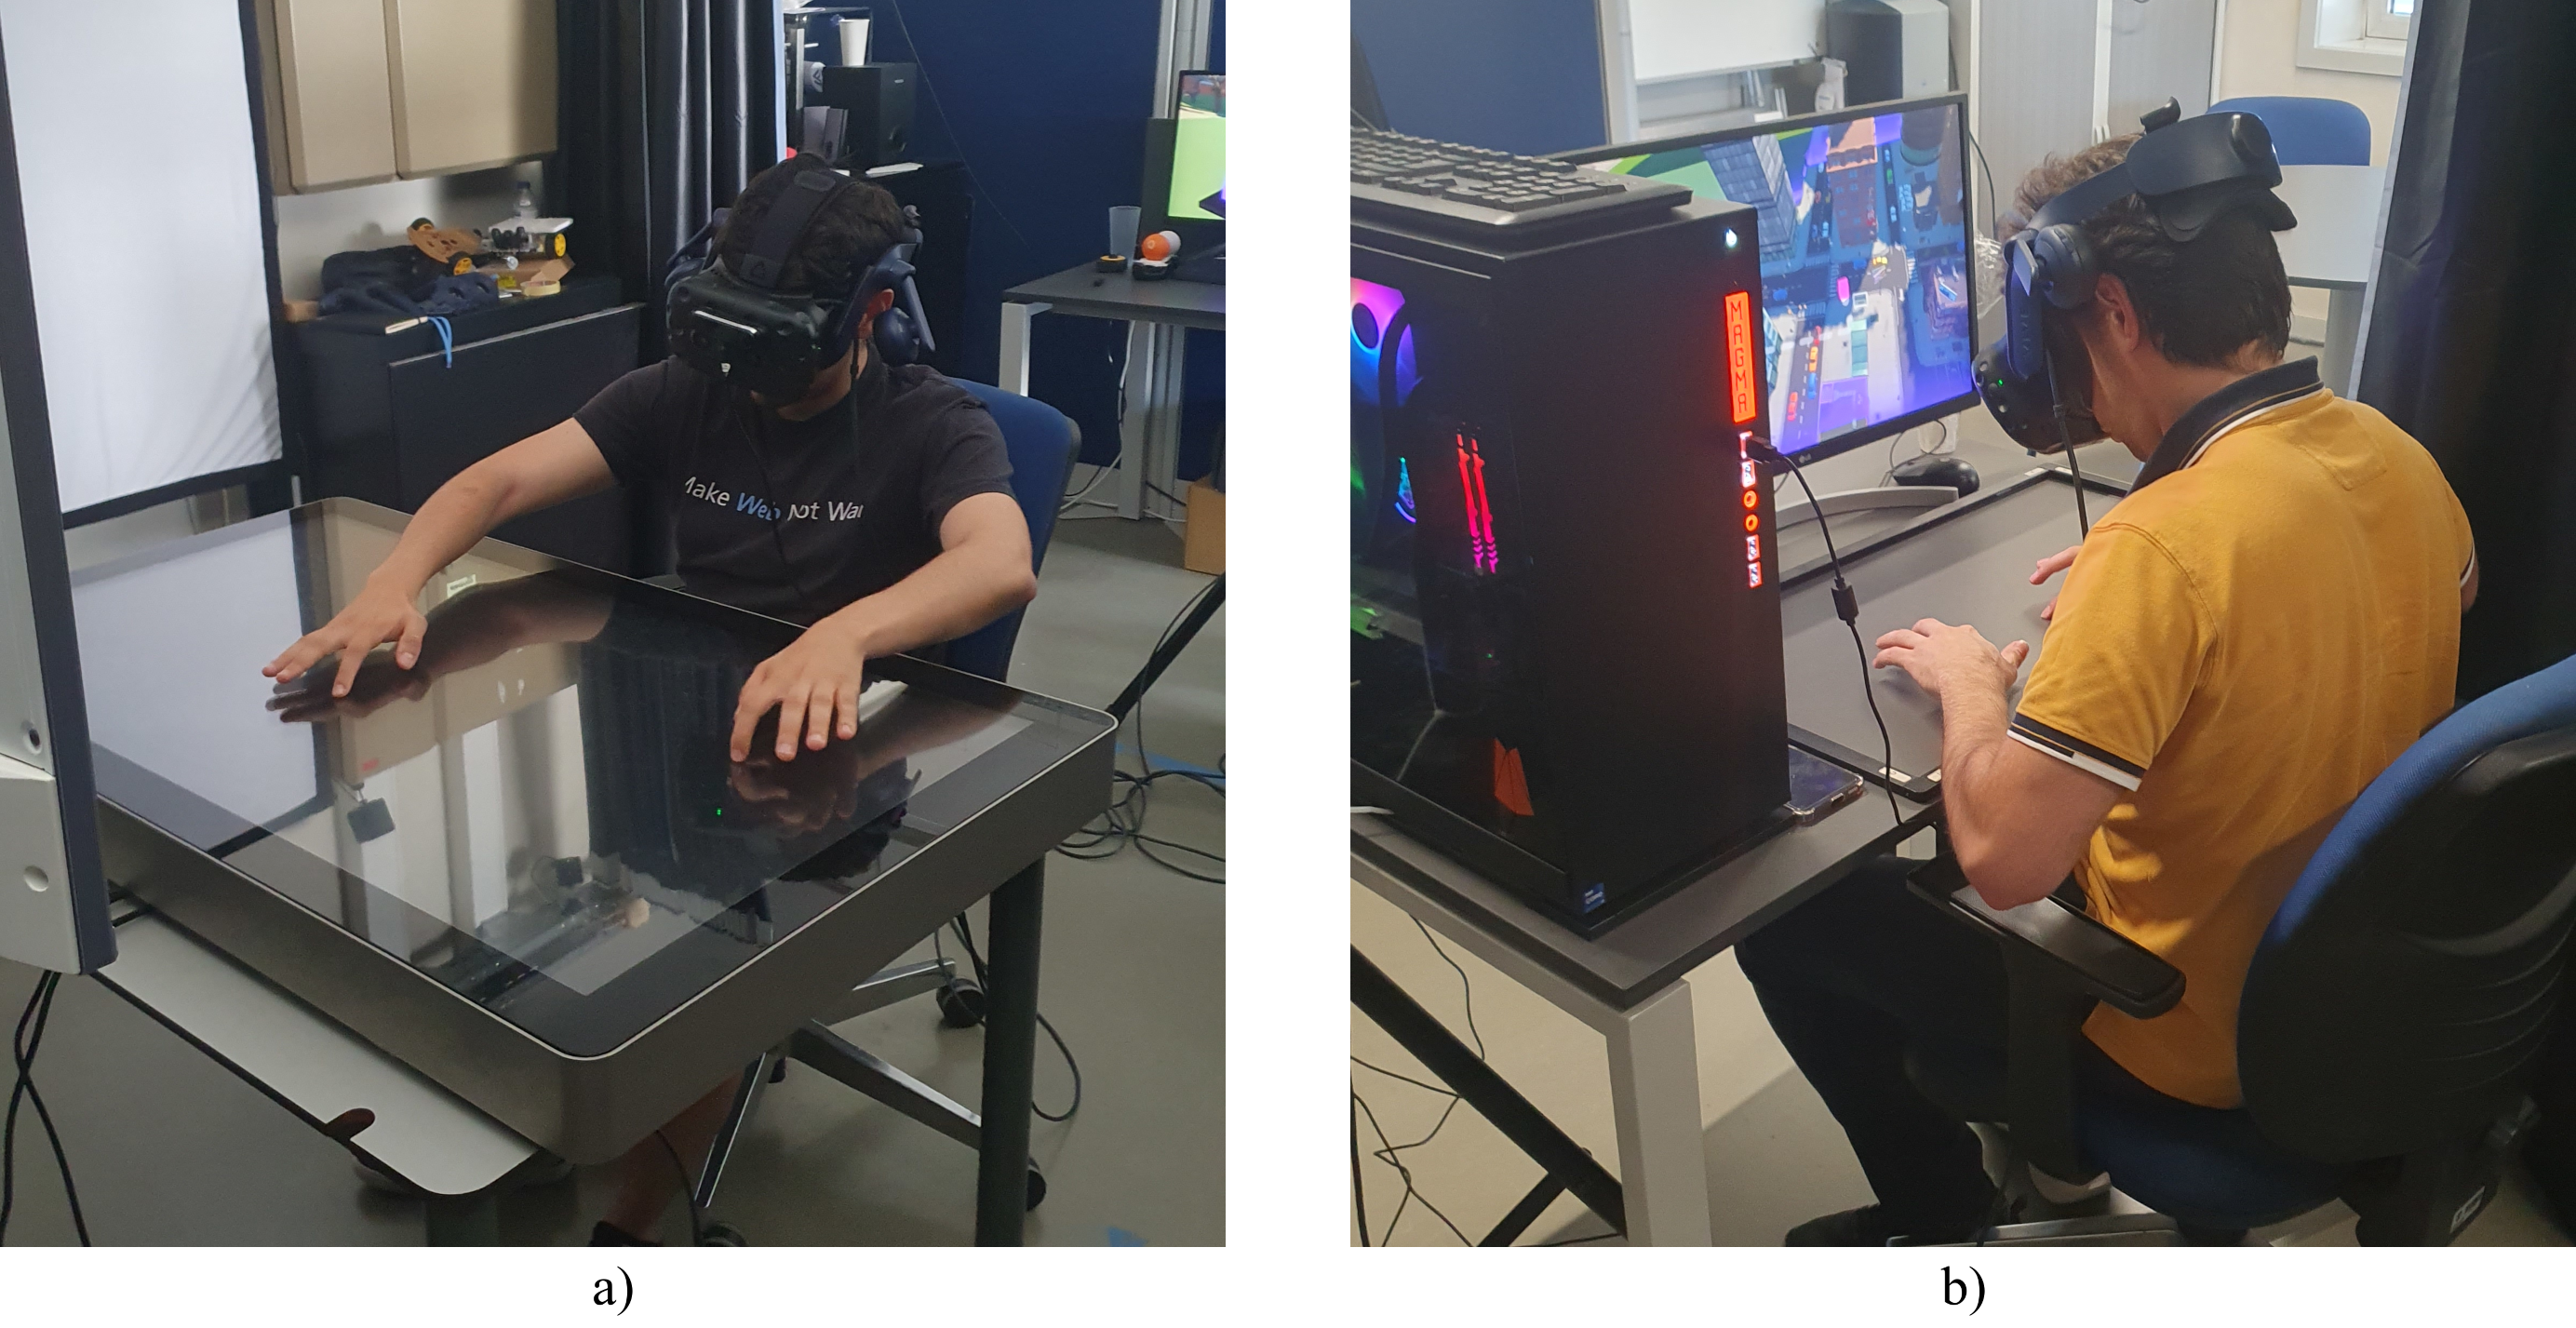
\includegraphics[width=1\linewidth]{figures/setup.png}
        \caption{Setup for the user study. In image (a) one participant is seated in front of the Displax Skin Ultra. In image (b) the participant is seated in front of the infrared touch frame.}
        \label{fig:eval_setup}
    \end{figure}

    One computer served as the host, while the other connected as a client. The setup process involved a starting screen where the moderator could select the IP address of the host computer. The roles of each computer did not change throughout the study to simplify the setup process and avoid confusion.

\section{Methodology}

    The study was conducted in pairs, with initial tasks performed individually and later tasks performed collaboratively. Each session consisted of three main parts: an introduction, a training session, and the main tasks. Each session lasted approximately 60 minutes. After each session, participants received a chocolate bar as a token of appreciation.

    Before the study began, participants were introduced briefly to the study's purpose and the Replico system. They then completed a consent form and a profiling questionnaire. Following this, they watched a video presentation explaining Replico's features, usage, and the tasks they would perform.

    During the training session, participants familiarized themselves with the system by experimenting with all of Replico's features. Once comfortable with the solo interactions, a set of points of interest and a simulated player were added to the environment, allowing users to practice acknowledging points of interest and joining the other user's table. After becoming comfortable with these interactions, they proceeded to the main tasks.

    The main tasks were performed using two different 3D models: a city and the Perseverance rover, described in Section \ref{sec:test_scenarios}. The order in which the models were used alternated between pairs to avoid bias. These tasks aimed to assess the efficiency and effectiveness of Replico's features, as described in Section \ref{sec:tasks}. Metrics for each task were collected as detailed in Section \ref{sec:evaluation_metrics}. Participants completed a questionnaire on the tasks they performed between each test scenario, described in Section \ref{sec:qualitative_data}.

    \subsection{Test Scenarios} \label{sec:test_scenarios}

        Three scenarios were used during the study, two for the main tasks, as shown in Figure \ref{fig:test_scenarios}. The first scenario, used for training, is a small dungeon tavern built with the free version of the KayKit Dungeon Remastered Pack from itch.io\footnote{\url{https://kaylousberg.itch.io/kaykit-dungeon-remastered}} and the Modular Asset Staging Tool (MAST) for Unity\footnote{\url{https://fertile-soil-productions.itch.io/mast}}. The second scenario is a city from Synty's POLYGON City Pack\footnote{\url{https://assetstore.unity.com/packages/3d/environments/urban/polygon-city-low-poly-3d-art-by-synty-95214}}, obtained through Unity's student plan. The third scenario features the Perseverance rover, obtained from NASA's 3D model repository\footnote{\url{https://nasa3d.arc.nasa.gov/detail/perseverance-glb}}, with the surrounding environment created using Unity's terrain tools and a tinted sand texture from Polyhaven\footnote{\url{https://polyhaven.com/a/sand_01}}.

        \begin{figure}[h]
            \centering
            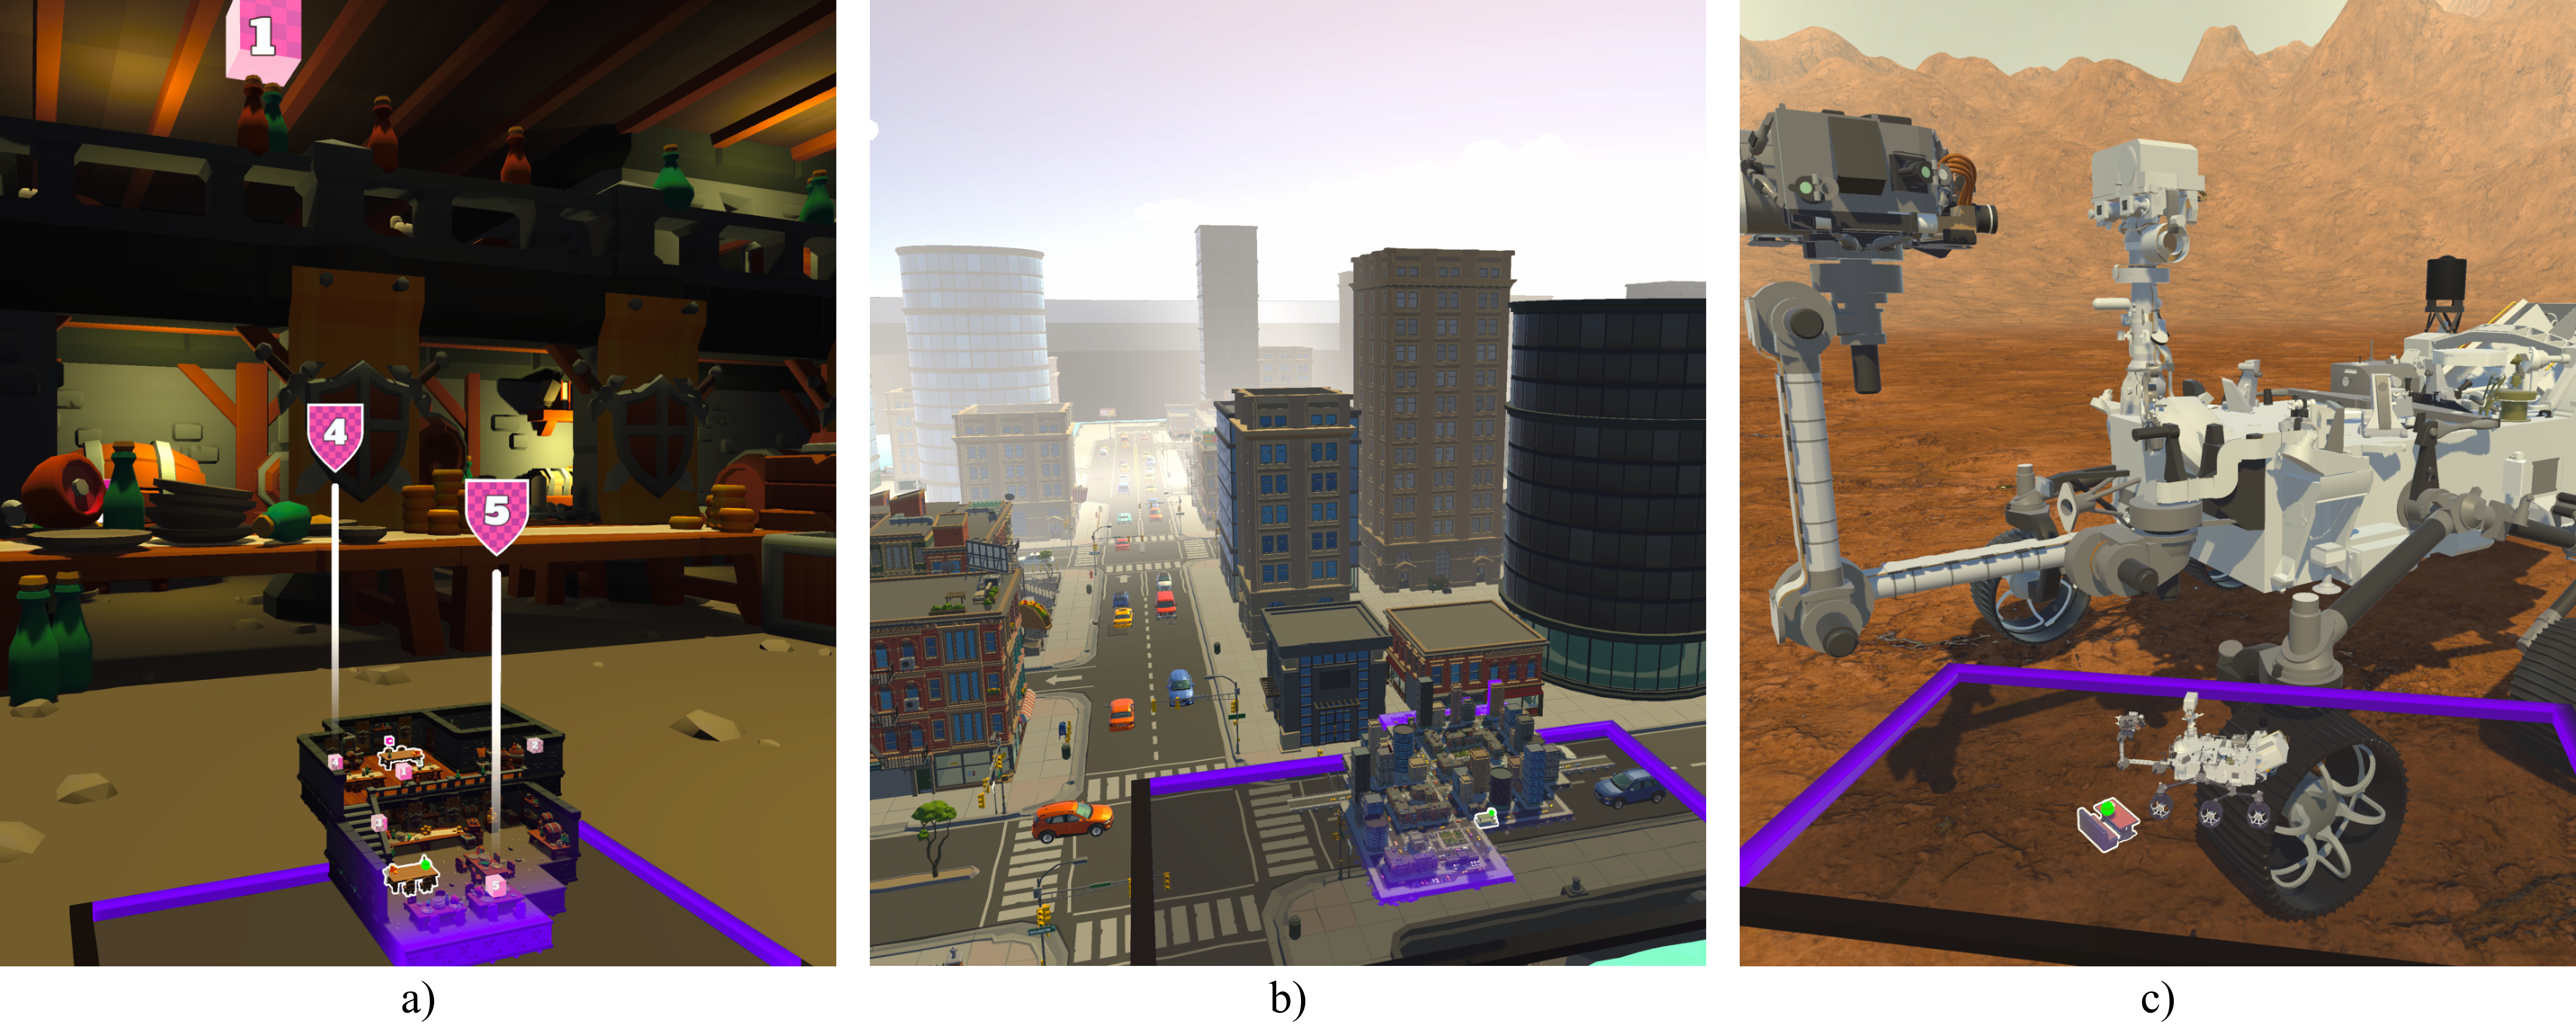
\includegraphics[width=1\linewidth]{figures/test_scenarios.png}
            \caption{The three test scenarios used in the user study. From left to right: the dungeon tavern, the city, and the Perseverance rover.}
            \label{fig:test_scenarios}
        \end{figure}

        Two scenarios were selected for the main tasks to evaluate how well the approach works with different 3D models. The city model was chosen for its large, complex structure, allowing users to immerse themselves within it. The Perseverance rover model was selected for its smaller size but sufficient detail, enabling users to view the entire model at once without being part of it. The dungeon tavern was used for practice, providing a small, enclosed environment distinct from the main task scenarios.

        In all scenarios, the virtual world includes surrounding environment elements to provide context and a sense of scale. For example, the city is bordered by an ocean, the rover by the Martian surface, and the dungeon tavern by some of its walls. The WIM does not replicate these environmental elements, as they are not part of the primary scenario.

    \subsection{Tasks} \label{sec:tasks}

        Participants performed five main tasks during the study, using each of the two main scenarios. The first three tasks were done individually, while the last two were collaborative. Each task evaluated different aspects of Replico's features and user experience. The tasks are as follows:

        \begin{itemize}
            \item \textbf{Task 1}: Create a point of interest on six different predefined objects in the scene. This task evaluates how efficiently users can create points of interest.
            \item \textbf{Task 2}: Acknowledge five out of twelve predefined points of interest created by a simulated user. This task assesses how effectively Replico notifies users of new points of interest.
            \item \textbf{Task 3}: Teleport to four different predefined zones and orient themselves to face a specific object. This task measures how well users can navigate the environment using Replico.
            \item \textbf{Task 4 \& 5}: One user must show another user a specific object in the scene without verbal communication. The other user then verbally confirms the object they believe the first user is referring to. Once confirmed, the roles are reversed, and the process is repeated with a different object. This task evaluates how well users can communicate points of interest using Replico
        \end{itemize}

        Between each task, the environment was reset to its initial state. Any points of interest created during the previous task were removed, and participants were placed back at their starting positions. This was done to ensure that each task was performed under the same conditions for all participants.

        In the first task, the predefined objects were chosen with different sizes and at various heights, visible in Figure \ref{fig:task_01}. The goal was to evaluate how efficiently users could create points of interest, not to test their ability to identify objects. To draw attention to them, these objects glowed with an expanding and contracting effect in the WIM. They increased in size and changed their outline color from white to green when the balloon intersected with them. Creating a point of interest during this state allowed users to progress to the next object. The objects appeared one at a time, immediately after the user created a point of interest on the previous object. The order in which the objects appeared was consistent for all participants.

        \begin{figure}[h!]
            \centering
            \includegraphics[width=1\linewidth]{figures/task_01.png}
            \caption{The six predefined objects used in Task 1 for each scenario. They are ordered from left to right, with the top row showing the objects in the city scenario while the bottom row shows the objects in the Perseverance rover scenario. The top-right image shows the green outline effect when the balloon intersects with the object.}
            \label{fig:task_01}
        \end{figure}

        In the second task, the predefined points of interest were placed around the environment simultaneously, as shown in Figure \ref{fig:task_02}. The goal was to evaluate how effectively Replico notifies users of new points of interest and helps distinguish acknowledged from unacknowledged points of interest. The task was complete when the user acknowledged the five unacknowledged points of interest. Participants could acknowledge the points of interest in any order.

        \begin{figure}[h!]
            \centering
            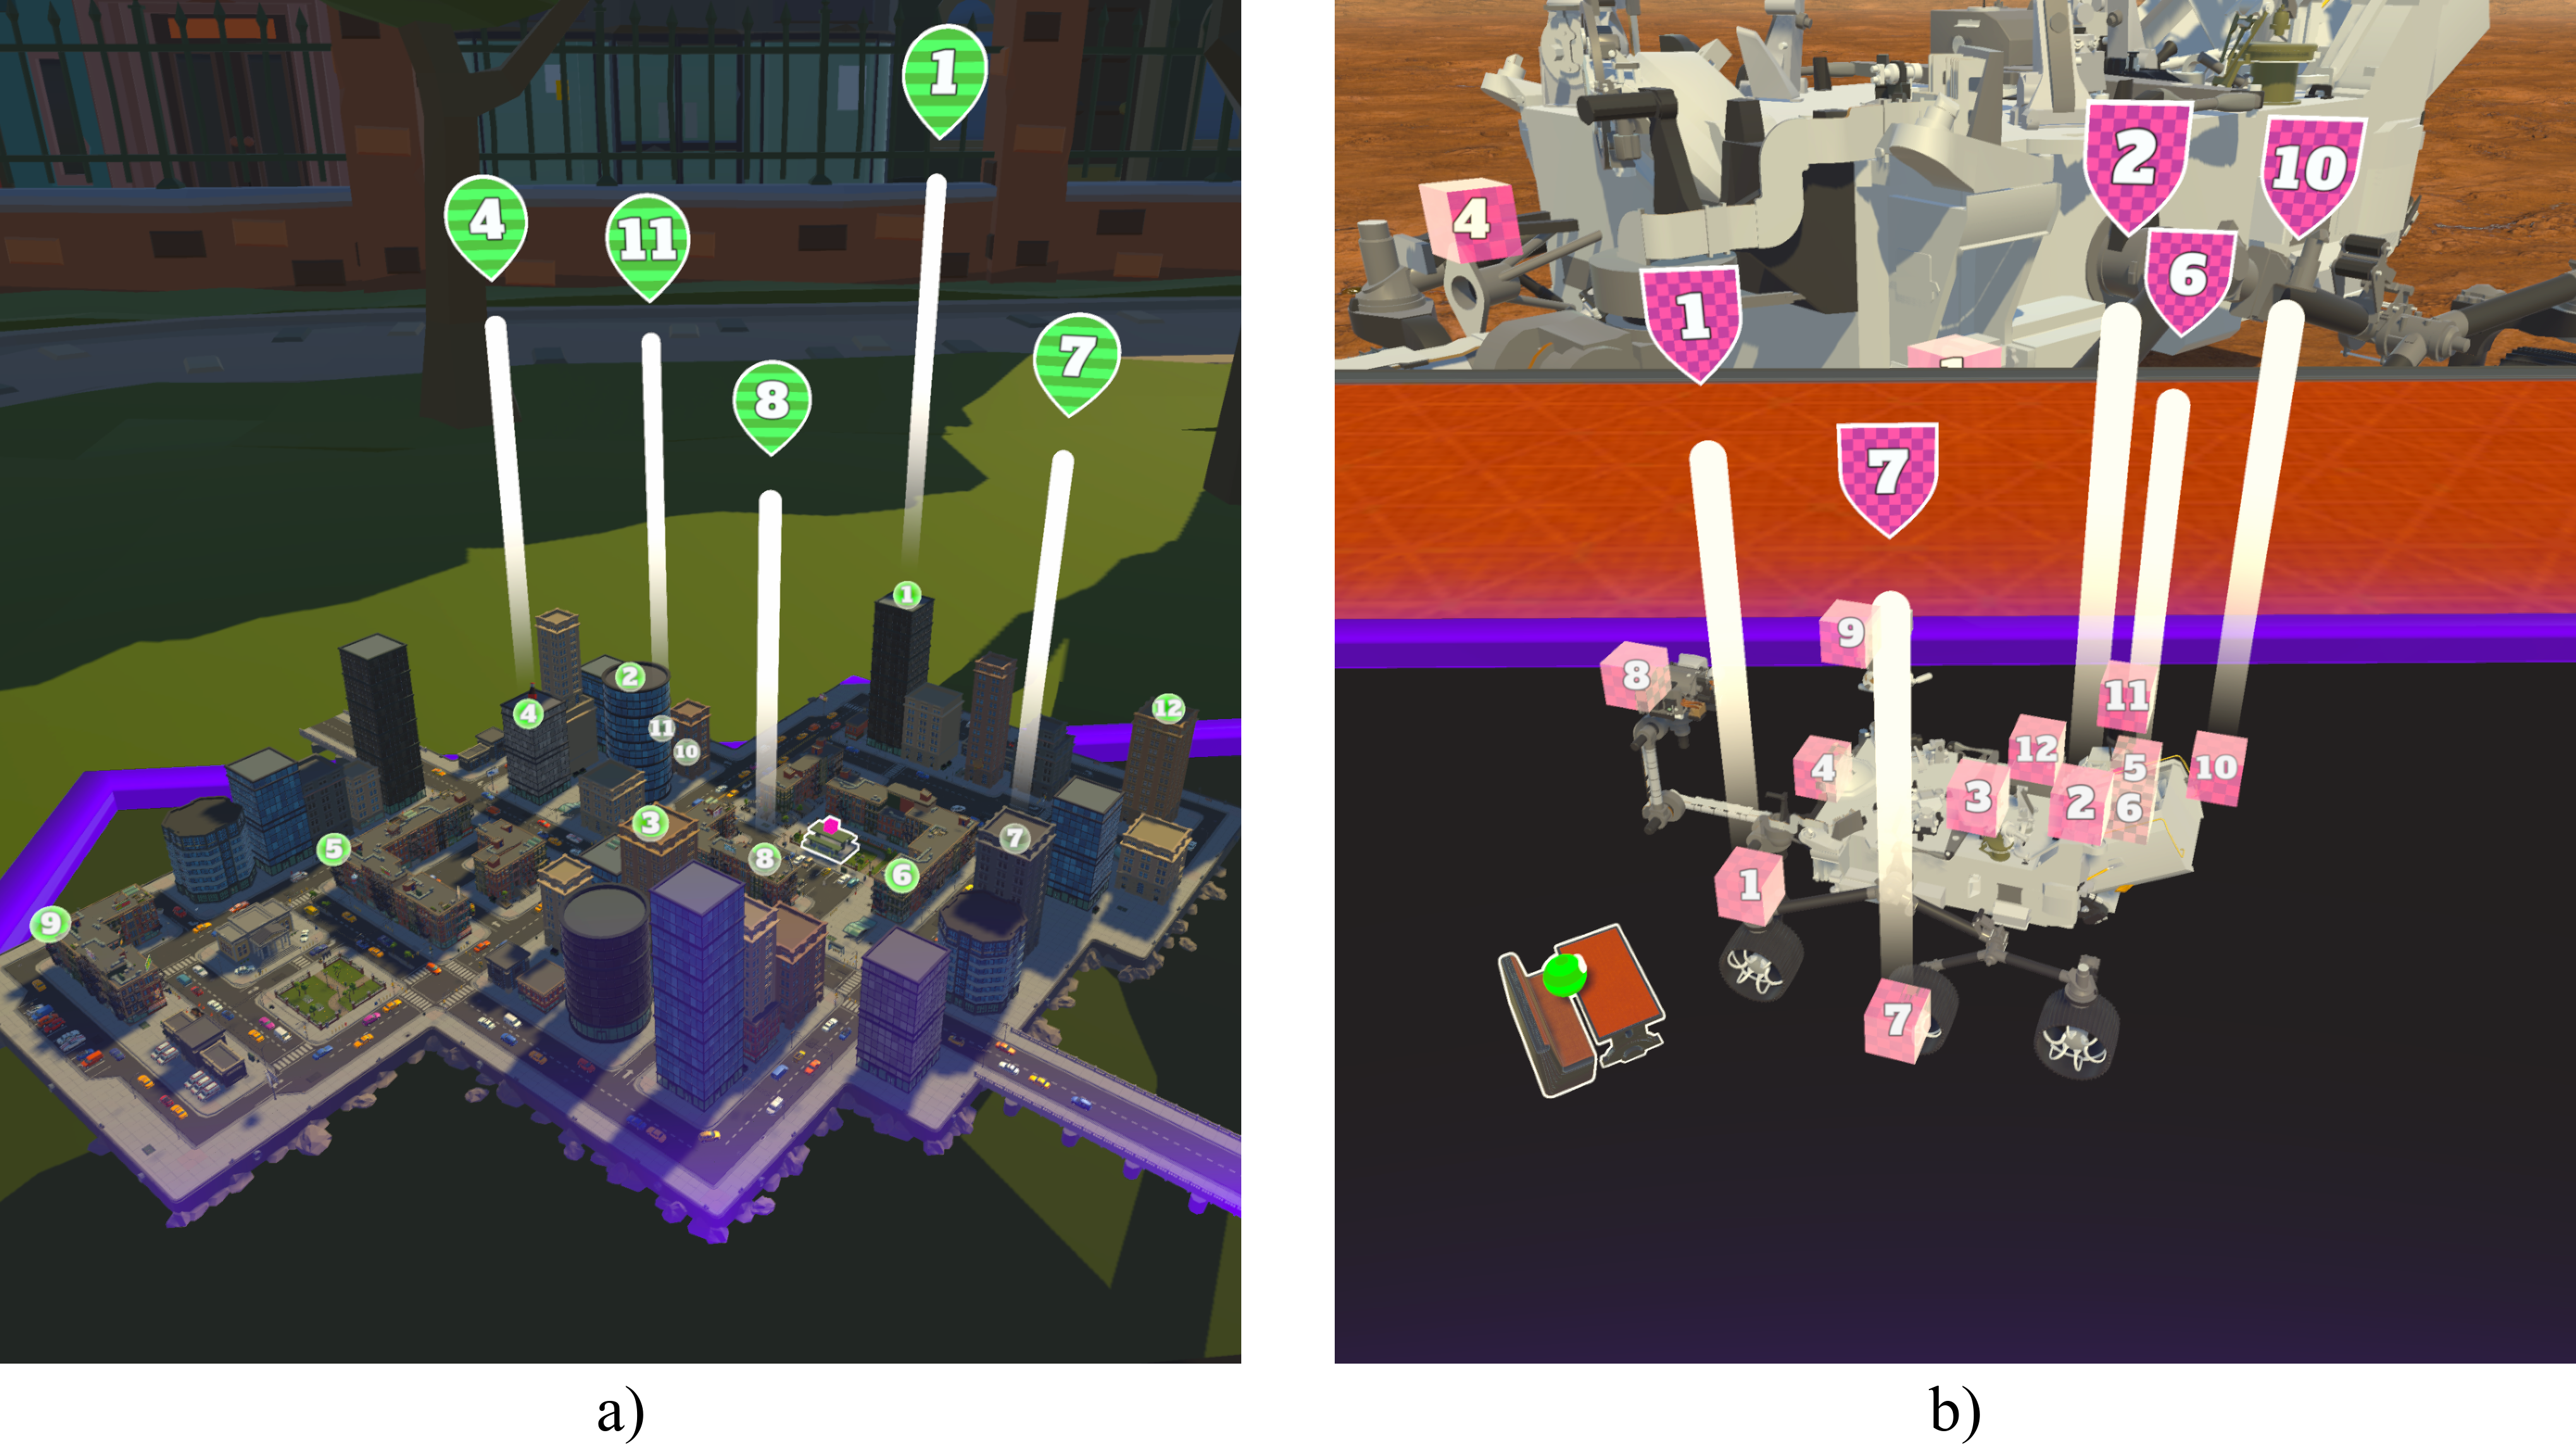
\includegraphics[width=1\linewidth]{figures/task_02.png}
            \caption{The created points of interest in Task 2. Image (a) shows the points of interest in the city scenario, while image (b) shows the points of interest in the Perseverance rover scenario.}
            \label{fig:task_02}
        \end{figure}

        In the third task, participants navigated through four predefined zones in the environment, as shown in Figure \ref{fig:task_03}. The goal was to assess how well users could navigate using Replico. Participants were instructed to teleport to each zone and orient themselves to face a specific object. Zones changed color from white to green when the balloon intersected with them, and the object's glow effect also changed from white to green when the user was correctly oriented. The moderator advanced the task manually, allowing participants to take their time exploring the environment. The sequence of zones was the same for all participants.

        \begin{figure}[h]
            \centering
            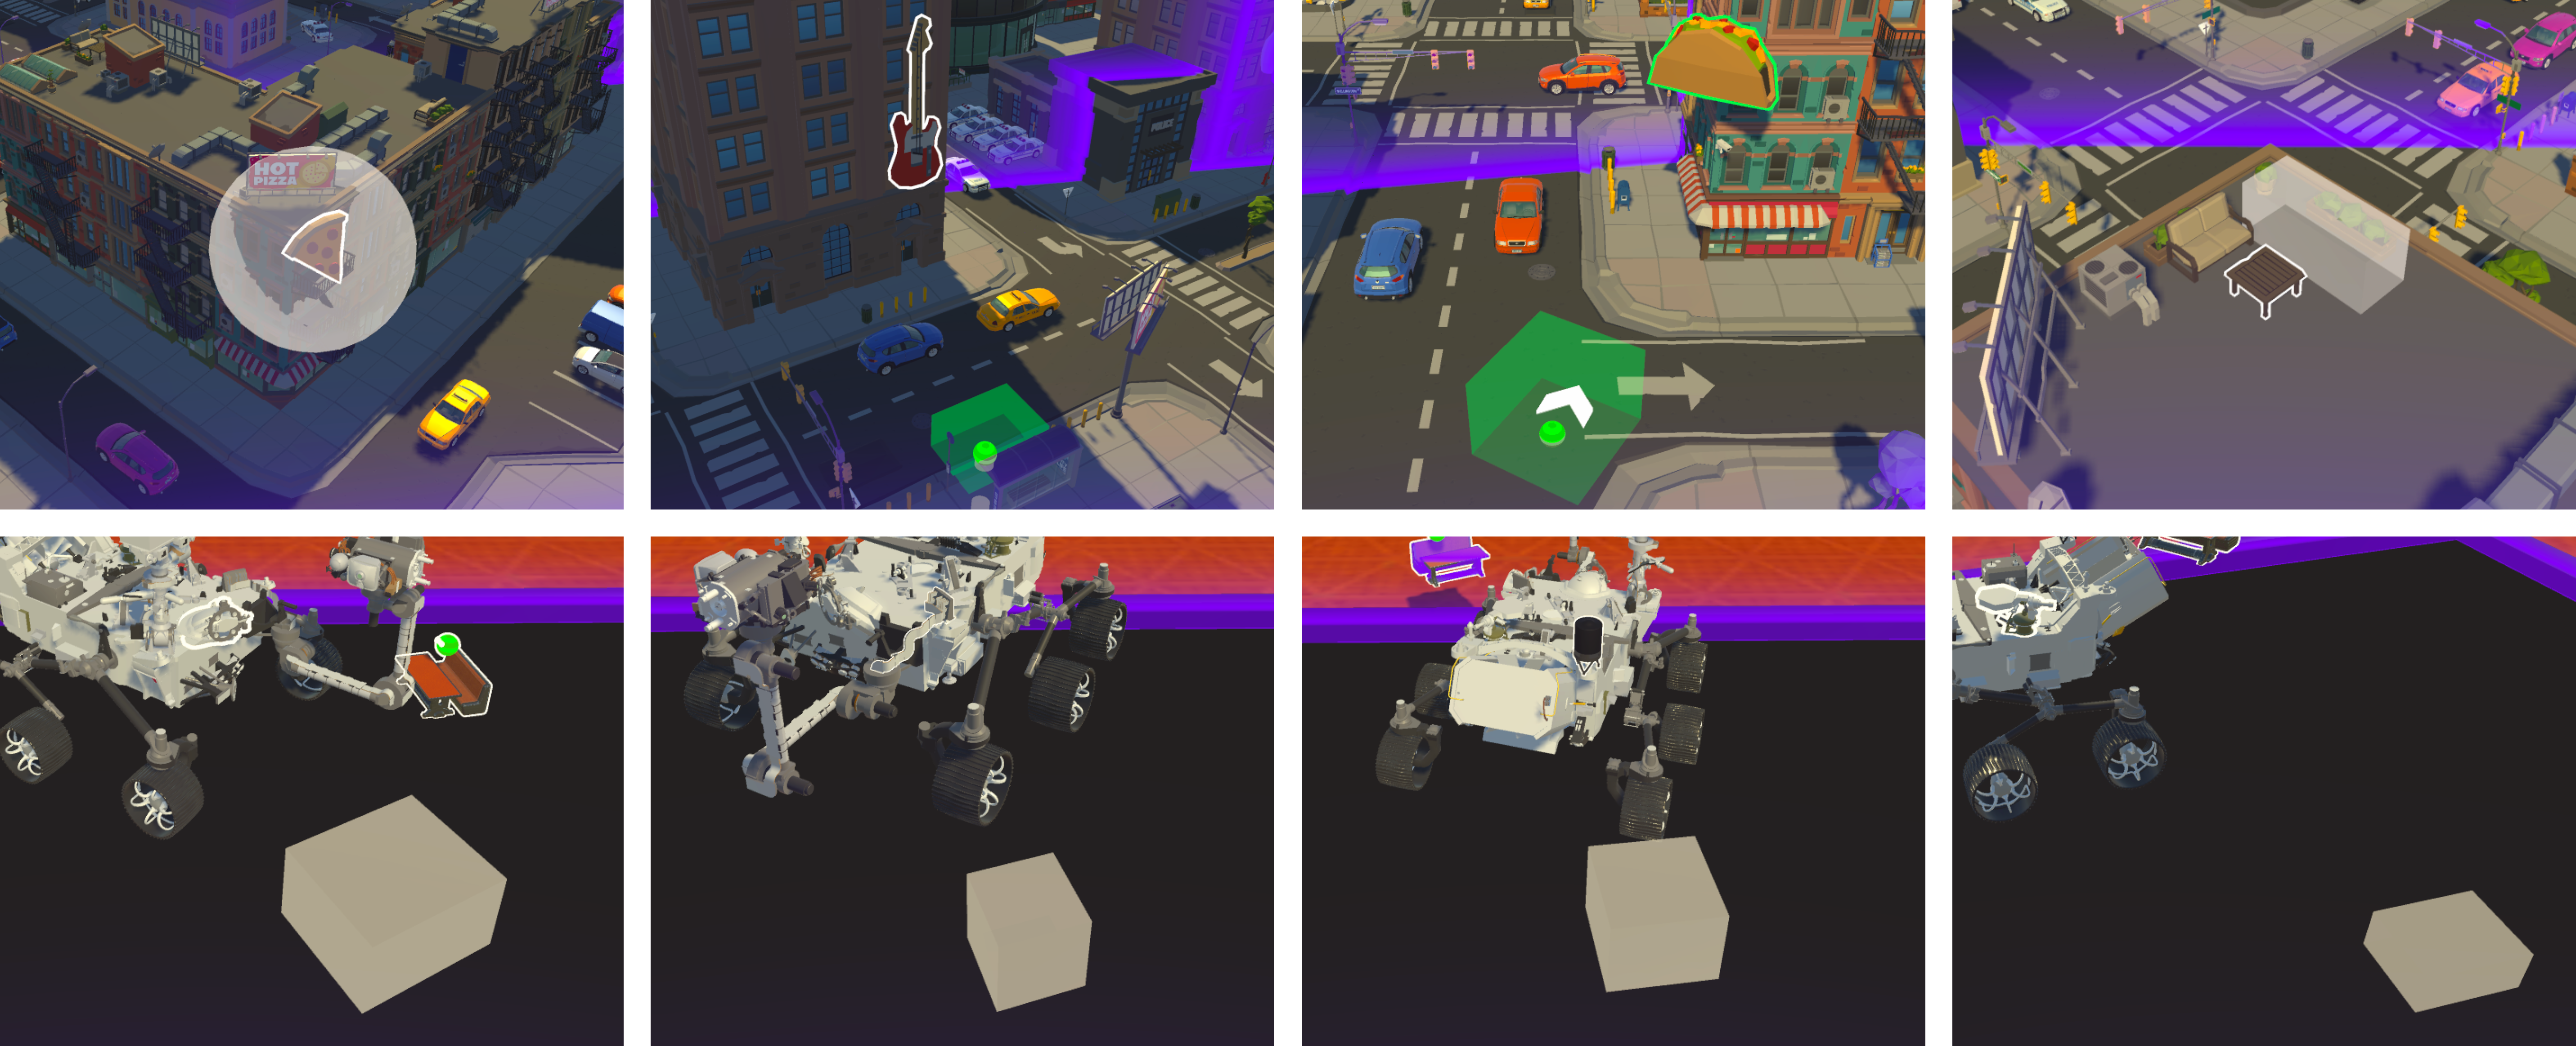
\includegraphics[width=1\linewidth]{figures/task_03.png}
            \caption{The four predefined zones used in Task 3 for each scenario. They are ordered from left to right, with the top row showing the zones in the city scenario while the bottom row shows the zones in the Perseverance rover scenario.}
            \label{fig:task_03}
        \end{figure}

        In the fourth and fifth tasks, participants communicated objects of interest without verbal communication. Figure \ref{fig:task_04} shows the objects used in these tasks. The goal was to assess how effectively users could communicate using Replico. The selected objects were small and difficult to identify from a distance, encouraging the use of the WIM, points of interest, and teleportation for effective communication. For the Perseverance rover model, since most people are unfamiliar with its components, the objects chosen were a small hidden star and a small hidden heart.

        \begin{figure}[h]
            \centering
            \includegraphics[width=1\linewidth]{figures/task_04.png}
            \caption{The objects used in Tasks 4 and 5 for each scenario. The top row shows the objects in the city scenario, while the bottom row shows the objects in the Perseverance rover scenario.}
            \label{fig:task_04}
        \end{figure}


    \subsection{Metrics} \label{sec:evaluation_metrics}

        During each task, several metrics were collected to evaluate the efficiency and effectiveness of Replico's features. These metrics, recorded automatically by the system, included the time in seconds taken to complete the task, the number of successful task steps, time spent transforming the replica, time spent in vertical transformation, and time spent in balloon selection. Additionally, the system tracked the number of times the transform gesture was detected (on entering \lstinline{TransformReplicaState}), the number of times vertical transform was detected (on entering \lstinline{TransformReplicaVerticalState}), and the number of times the balloon selection gesture was detected (on entering \lstinline{BalloonSelectionInitialState}). It also recorded the number of points of interest created, deleted, and acknowledged, the number of teleportations, the number of table joins, the number of touches on the touch surface, the cumulative sum of finger movement in pixels, the cumulative sum of head rotation in angles, cumulative head translation in meters, cumulative sum of replica rotation in angles, cumulative sum of replica translation in meters, and cumulative sum of replica scaling in meters.

        The time taken to complete each task was measured from the start to the end of the task. In Task 3, while the participant waited for the moderator to advance to the next zone, all metrics were paused. The number of successful task steps was the number of steps completed correctly by the user. For example, in Task 1, a successful step was creating a point of interest on a predefined object. In Task 2, a successful step was acknowledging a point of interest. In Task 3, a successful step was teleporting to a zone and orienting oneself to face a specific object. In Tasks 4 and 5, it referred to the number of guesses until the correct object was identified.

        Additionally, data was collected and timestamped for each frame that showed a change. This included finger data, replica transform data, and head transform data.
    
    \subsection{Qualitative Data} \label{sec:qualitative_data}

        After each test scenario, participants completed a questionnaire to provide qualitative feedback on their experience. The questionnaire included six questions from the NASA Task Load Index (NASA-TLX) \cite{hart1988development} for each task, merging tasks 4 and 5 into a single task, along with three additional questions at the end of the questionnaire, each rated on a 5-point Likert scale. The NASA-TLX questions were:

        \begin{itemize}
            \item How mentally demanding was the task?
            \item How physically demanding was the task?
            \item How hurried or rushed was the pace of the task?
            \item How successful were you in accomplishing what you were asked to do?
            \item How hard did you have to work to accomplish your level of performance?
            \item How insecure, discouraged, irritated, stressed, and annoyed were you?
        \end{itemize}

        The final three questions were:

        \begin{itemize}
            \item How nauseous did you feel during the task?
            \item How useful was the world-in-miniature metaphor for communicating points of interest?
            \item How useful was the representation of user locations on the replica for understanding intent?
        \end{itemize}

        Participants were also encouraged to provide additional comments or suggestions for improvement. The aim was to gather feedback on the user experience and identify areas for improvement in the system.

\section{Participants}

    A total of 20 participants, forming ten pairs, took part in the study. Among them, eleven were male, and nine were female. Most participants, 19, were aged between 21 and 30 years old, with one participant aged between 31 and 40. Nineteen participants were right-handed, and one was left-handed. Seventeen participants were students, of whom six also worked, while three were exclusively workers. Fifteen participants had completed a bachelor's degree, two had a master's degree, and three had a high school diploma. Regarding VR experience, 11 had used VR once before, three had used it in the past year, one used it frequently, and five had never used VR before.

\section{Results}

    The results of the user study are presented in this section. Two samples were collected for each task metric, one for each test scenario. Appropriate statistical tests were performed to determine the significance of the results, with the significance level set at the conventional alpha value of 5\%.

    \subsection{Metrics}

        Using descriptive data analysis, outliers were identified and removed from the dataset. The Shapiro-Wilk test \cite{shapiroAnalysisVarianceTest1965} was used to determine if the data followed a normal distribution. Since the analysis involved testing two related samples, either the paired t-test or the Wilcoxon signed-rank test \cite{wilcoxonIndividualComparisonsRanking1945} was used to determine whether the samples' differences were statistically significant. The paired t-test was used for normally distributed data, while the Wilcoxon signed-rank test was used for non-normally distributed data.

        For the metrics of task 4 and task 5, except for task completion time (which was the same for both participants), the metrics were split into two separate tasks: one for the seeker (TaskSeek) and one for the shower (TaskShow). A two-way repeated measures ANOVA with Bonferroni correction was used to determine if there were significant differences between two factors: the object (task 4 or task 5) and the scenario (city or rover). If the sphericity assumption was violated according to Mauchly's test of sphericity, the Greenhouse-Geisser correction was applied. If the interaction effect was significant, a simple main effects analysis was performed to identify the specific differences. The studentized residuals were checked for outliers, and the data was checked for normality to ensure the assumptions of the ANOVA were met.

        Five metrics were selected for analysis: task completion time, active time, finger movement, replica translation, and head translation. The results for each metric are presented in the following sections.

        \subsubsection{Task Completion Time}

            % task1city follows a normal distribution (p = .128)
            % task2city follows a normal distribution (p = .268)
            % task3city does not follow a normal distribution (p=.004) --!
            % task4city does not follow a normal distribution (p=.005)
            % task5city does not follow a normal distribution (p=.002)
            % task1rover follows a normal distribution (p = .064)
            % task2rover follows a normal distribution (p = .735)
            % task3rover follows a normal distribution (p = .580) -- !
            % task4rover does not follow a normal distribution (p=.026)
            % task5rover does not follow a normal distribution (p=.012)

            \begin{figure}[h!]
                \centering
                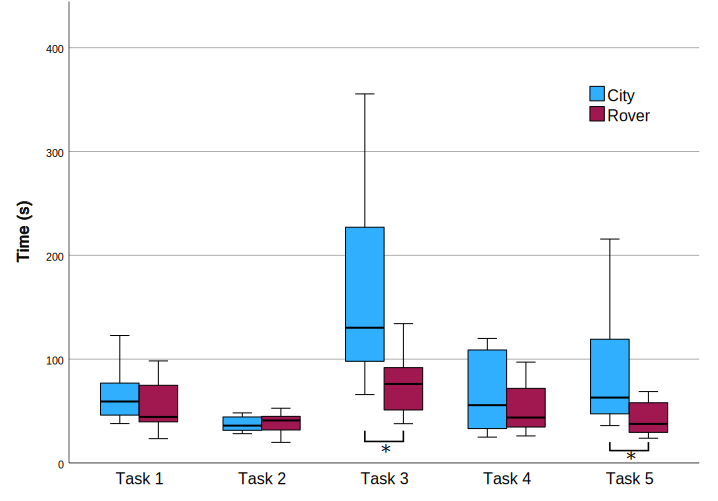
\includegraphics[width=1\linewidth]{figures/task_time_graph.pdf}
                \caption{Box-plot of the time taken to complete each task for each scenario. The symbol $\ast$ indicates a significant difference between the city and rover scenarios.}
                \label{fig:task_time}
            \end{figure}

            Task completion time, recorded in seconds, measures how long it took participants to complete each task. The results for each task are shown in Figure \ref{fig:task_time}. For the first task, there was no significant difference in completion time between the city and rover scenarios ($t(14) = 1.440,\ p = 0.172$). Similarly, the second task showed no significant difference in completion time between the two scenarios ($t(10) = 0.134,\ p = 0.896$). However, for the third task, there was a significant difference in completion time between the two scenarios ($Z = -3.248,\ p = 0.001$), with participants taking longer in the city scenario. The fourth task also showed no significant difference in completion time between the two scenarios ($Z = -1.415,\ p = 0.157$). The fifth task had a significant difference in completion time between the two scenarios ($Z = -3.154,\ p = 0.002$), with participants taking longer in the city scenario.

            Overall, task completion times were similar between the city and rover scenarios, except for tasks 3 and 5. Task 3 took longer in the city scenario, likely due to the difficulty of locating the teleportation zones. These zones were more spread out and smaller, making balloon selection harder and requiring participants to be more precise. Although participants could scale the replica to aid selection, they generally did not. Task 5 also took longer in the city scenario because the shower object was small and hidden among other objects, making it harder for the seeker to find. 
            
            In contrast, in the rover scenario, the objects were easier to locate, with some participants finding them by accident during previous tasks. Additionally, points of interest in the WIM are visible behind objects, which can completely obscure small objects. Teleportation would help in this case, as points of interest in the to-scale model aren't visible behind objects and become smaller as the user gets closer to them. However, participants generally did not use it.

        \subsubsection{Active Time}

            % task1city p = .042: does not follow a normal distribution
            % task2city p = .572: follows a normal distribution
            % task3city p=.005: does not follow a normal distribution
            % task1rover p = .068: follows a normal distribution
            % task2rover p = .802: follows a normal distribution
            % task3rover p = .209: follows a normal distribution
   
            \begin{figure}[h!]
                \centering
                \includegraphics[width=1\linewidth]{figures/active_time_graph.pdf}
                \caption{Box plot showing the active time for each task in both scenarios. The asterisk ($\ast$) indicates a significant difference between the city and rover scenarios. The dagger ($\dag$)  shows significant differences between objects in TaskSeek and TaskShow.}
                \label{fig:active_time}
            \end{figure}

            Active time, measured in seconds, represents the duration participants spent actively touching the touch surface. The results for each task are shown in Figure \ref{fig:active_time}. In the first task, there was no significant difference in active time between the city and rover scenarios ($t(12) = -1.913,\ p = 0.056$). The second task also showed no significant difference in active time between the two scenarios ($t(12) = -1.431,\ p = 0.178$). However, for the third task, participants spent significantly more active time in the city scenario ($Z = -3.051,\ p=0.002$).

            A repeated measures ANOVA with Greenhouse-Geisser correction revealed no significant difference in active time between the different scenarios in TaskSeek ($F(1, 9) = 4.680,\ p = 0.059$), and no significant difference between the different objects ($F(1, 9) = 2.468,\ p = 0.151$). However, the scenarios and objects had a significant interaction effect ($F(1, 9) = 12.630,\ p = 0.006$). Simple main effects analysis showed that, in the city scenario, there was a significant difference in active time between the different objects ($p=0.035$), with the second object having a significantly higher active time. In the rover scenario, there was no significant difference in active time between the different objects ($p=0.075$). For the first object, there was no significant difference in active time between the city and rover scenarios ($p=0.767$). However, for the second object, there was a significant difference in active time between the city and rover scenarios ($p=0.017$).

            A repeated measures ANOVA with Greenhouse-Geisser correction also determined no significant difference in active time between the different scenarios in TaskShow ($F(1, 6) = 4.472,\ p = 0.079$), and no significant difference between the different objects ($F(1, 6) = 3.217,\ p = 0.123$). However, the scenarios and objects had a significant interaction effect ($F(1, 6) = 16.370,\ p = 0.007$). Simple main effects analysis revealed that, in the city scenario, there was a significant difference in active time between the different objects ($p=0.032$), with the second object having a significantly higher active time. In the rover scenario, there was no significant difference in active time between the different objects ($p=0.429$). For the first object, there was no significant difference in active time between the city and rover scenarios ($p=0.935$). However, for the second object, there was a significant difference in active time between the city and rover scenarios ($p=0.025$).

            Compared to task completion time, active time was mainly comparable between the city and rover scenarios, except for Task 3, Task 5 Seek, and Task 5 Show, where participants spent more active time in the city scenario. This analysis highlights the increased difficulty of the second object compared to the first object in the collaborative tasks for the city scenario. Both objects were equally challenging to find in the rover scenario, with participants spending similar active time on both.

        \subsubsection{Finger Movement}

            % task1city p = .455: follows a normal distribution
            % task2city p = .2: follows a normal distribution
            % task3city p =.045: does not follow a normal distribution
            % task4seekCity p =.409: follows a normal distribution
            % task4showCity p =.479: follows a normal distribution
            % task5seekCity p =.621: follows a normal distribution
            % task5showCity p =.018: does not follow a normal distribution
            % task1rover p = .323: follows a normal distribution
            % task2rover p = .801: follows a normal distribution
            % task3rover p = .255: follows a normal distribution
            % task4seekRover p = .358: follows a normal distribution
            % task4showRover p = .582: follows a normal distribution
            % task5seekRover p = .177: follows a normal distribution
            % task5showRover p = .921: follows a normal distribution

            \begin{figure}[h!]
                \centering
                \includegraphics[width=1\linewidth]{figures/finger_movement_graph.pdf}
                \caption{Box plot showing the cumulative sum of finger movement in meters for each task in both scenarios. The asterisk ($\ast$) indicates a significant difference between the city and rover scenarios.}
                \label{fig:finger_movement}
            \end{figure}

            Finger movement, measured in meters, represents the cumulative distance traveled by participants' fingers on the touch surface. Each touch surface's pixels per inch (PPI) was calculated using its dimensions and screen resolution to convert pixel data to meters. The pixel finger movement data was then divided by the PPI to convert it to inches, and this value was subsequently converted to meters. The results for each task are shown in Figure \ref{fig:finger_movement}. 

            In the first task, there was a significant difference in finger movement between the city and rover scenarios ($t(14) = 2.976,\ p = 0.010$), with participants moving their fingers more in the city scenario. The second task showed no significant difference in finger movement between the two scenarios ($t(15) = 1.030,\ p = 0.320$). However, for the third task, there was a significant difference in finger movement between the city and rover scenarios ($Z = -3.285,\ p = 0.001$), with participants again moving their fingers more in the city scenario.

            A repeated measures ANOVA with Greenhouse-Geisser correction revealed a significant difference in finger movement between the different scenarios in TaskSeek ($F(1, 5) = 9.907,\ p = 0.025$), with participants moving their fingers more in the city scenario. There was no significant difference in finger movement between the different objects ($F(1, 5) = 2.048,\ p = 0.212$), and no significant interaction effect between the scenarios and objects ($F(1, 9) = 0.976,\ p = 0.368$). For TaskShow, there was a significant difference in finger movement between the different scenarios ($F(1, 6) = 6.409,\ p = 0.045$), with participants moving their fingers more in the city scenario. There was no significant difference in finger movement between the different objects ($F(1, 6) = 4.822,\ p = 0.070$), and no significant interaction effect between the scenarios and objects ($F(1, 6) = 5.897,\ p = 0.050$).

            Participants moved their fingers more in the city than in the rover scenario, except for Task 2. This increased movement is likely due to the city's more extensive and complex environment, where objects of interest are more spread out, necessitating more exploration and finger movement for transform gestures. The minimal difference in finger movement in Task 2 might be attributed to the fact that points of interest do not scale with the replica, making them easier to recognize without scaling, as they remain the same size.

        \subsubsection{Replica Translation}

            % task1city p = .003: does not follow a normal distribution
            % task2city p = .066: follows a normal distribution
            % task3city p = .095: follows a normal distribution
            % task1rover p = .354: follows a normal distribution
            % task2rover p = .185: follows a normal distribution
            % task3rover p = .234: follows a normal distribution
            
            \begin{figure}[h!]
                \centering
                \includegraphics[width=1\linewidth]{figures/replica_translation_graph.pdf}
                \caption{Box-plot of the cumulative sum of replica translation in meters for each task for each scenario. The asterisk ($\ast$) indicates a significant difference between the city and rover scenarios.}
                \label{fig:task_time}
            \end{figure}

            Replica translation, measured in meters, represents the cumulative distance participants moved the replica. The results for each task are shown in Figure \ref{fig:task_time}. All tasks showed a significant difference in replica translation between the city and rover scenarios, with participants moving the replica more in the city scenario (Task 1: $Z = -3.058,\ p = 0.002$; Task 2: $t(16) = 3.594,\ p = 0.002$; Task 3: $t(16) = 6.724,\ p < 0.001$).

            A repeated measures ANOVA with Greenhouse-Geisser correction revealed a significant difference in replica translation between the different scenarios in TaskSeek ($F(1, 4) = 34.498,\ p = 0.004$), with participants moving the replica more in the city scenario. There was no significant difference in replica translation between the different objects ($F(1, 4) = 4.246,\ p = 0.108$) and no significant interaction effect between the scenarios and objects ($F(1, 4) = 3.742,\ p = 0.125$). For TaskShow, there was a significant difference in replica translation between the different scenarios ($F(1, 7) = 21.834,\ p = 0.002$), with participants moving the replica more in the city scenario. There was no significant difference in replica translation between the different objects ($F(1, 7) = 3.039,\ p = 0.125$) and no significant interaction effect between the scenarios and objects ($F(1, 7) = 4.955,\ p = 0.065$).

            Like finger movement, participants moved the replica more in the city than in the rover scenario. However, unlike finger movement, this difference was evident across all tasks, including Task 2. This discrepancy may be due to the primary interaction in Task 2 being the acknowledgment of points of interest, which requires the use of two fingers for balloon selection. In contrast, replica translation can be done with one finger, meaning replica translation may not have impacted finger movement as much as acknowledging points of interest did.

        \subsubsection{Head Translation}

            % task1city p = 0.902: follows a normal distribution
            % task2city p = 0.157: follows a normal distribution
            % task3city p = 0.013: does not follow a normal distribution
            % task1rover p = 0.425: follows a normal distribution
            % task2rover p = 0.007: does not follow a normal distribution
            % task3rover p = 0.443: follows a normal distribution    

            \begin{figure}[h!]
                \centering
                \includegraphics[width=1\linewidth]{figures/head_graph.pdf}
                \caption{Box-plot of the cumulative head translation in meters for each task for each scenario.}
                \label{fig:task_time}
            \end{figure}

            Head translation, measured in meters, indicates the total distance participants moved their heads. Figure \ref{fig:task_time} displays the results for each task. In the first task, there was no significant difference in head translation between the city and rover scenarios ($t(9) = 0.550,\ p = 0.298$). Similarly, the second task showed no significant difference ($Z = -1.870,\ p = 0.062$). However, in the third task, participants moved their heads significantly more in the city scenario compared to the rover scenario ($Z = -2.427,\ p = 0.015$).

            A repeated measures ANOVA with Greenhouse-Geisser correction identified a significant difference in head translation across scenarios in TaskSeek ($F(1, 5) = 7.679,\ p = 0.039$), with more significant head movement observed in the city scenario. There was no significant difference in head translation between different objects ($F(1, 5) = 4.505,\ p = 0.087$), but an interaction effect between scenarios and objects was significant ($F(1, 5) = 7.237,\ p = 0.043$). To interpret this interaction, simple main effects analyses were conducted: head translation did not significantly differ across objects in the city scenario ($p = 0.064$) or the rover scenario ($p = 0.799$). Specifically, the head movement did not significantly differ between the city and rover scenarios for the first object ($p = 0.106$) but did for the second object ($p = 0.040$).

            In TaskShow, a repeated measures ANOVA indicated a significant difference in head translation between scenarios ($F(1, 5) = 10.181,\ p = 0.025$), with more head movement observed in the city scenario. There was no significant difference in head translation across different objects ($F(1, 5) = 4.445,\ p = 0.089$), nor was there a significant interaction effect between scenarios and objects ($F(1, 5) = 6.043,\ p = 0.057$).

            Overall, participants generally moved their heads more in the city scenario compared to the rover scenario, except for tasks 1 and 2, and Task 4 Seek.

    \subsection{Qualitative Data}

        The results from the questionnaires are discrete, ordinal data, as opposed to the continuous data from the metrics. As such, the Wilcoxon signed-rank test was used to determine if significant differences existed between the responses for each question across scenarios.

        Table \ref{tab:analysis_qualitative_1} displays the results for the first task. No significant differences were found between the city and rover scenarios for any of the questions. This suggests a similar task load in both scenarios. Participants generally did not report feeling mentally or physically strained, rushed, or insecure. They also felt successful in accomplishing their tasks and believed their performance required a lower-to-moderate level of effort.
       
        \begin{table}[h!]
            \caption{Median (IQR) and Wilcoxon Signed Ranks test results for each of the NASA-TLX questions for the first task in each scenario.}
            \begin{tabularx}{1\textwidth}{X l l l}
                \hline
                \multirow{2}{*}{Question} & \multicolumn{2}{c}{Median (IQR)} & \multirow{2}{*}{Wilcoxon Signed Ranks} \\
                \cline{2-3}
                & \makecell{City} & \makecell{Rover} &  \\
                \hline
                \hline
                How mentally demanding was the task? & 2 (1) & 1 (1) & $Z = -0.977,\ p = 0.329$ \\
                How physically demanding was the task? & 1 (1) & 1 (0.75) & $Z = -0.322,\ p = 0.748$  \\
                How hurried or rushed was the pace of the task? & 2 (1.75) & 1 (2) & $Z = -1.578,\ p = 0.115$\\
                How successful were you in accomplishing what you were asked to do? & 5 (1) & 5 (0.75) & $Z = -1.100,\ p = 0.271$ \\
                How hard did you have to work to accomplish your level of performance? & 2 (1.75) & 2 (2) & $Z = -0.844,\ p = 0.399$ \\
                How insecure, discouraged, irritated, stressed, and annoyed were you? & 1 (1) & 1 (0.75) & $Z = -0.551,\ p = 0.582$ \\
            \end{tabularx}
            \label{tab:analysis_qualitative_1}
        \end{table}
  
        Table \ref{tab:analysis_qualitative_2} presents the results for the second task. The city scenario was statistically significantly more demanding than the rover scenario regarding the effort required to achieve the performance level ($Z = -2.055,\ p = 0.040$). No other significant differences were observed between the two scenarios. Participants did not indicate feeling mentally or physically strained, rushed, or insecure in either scenario. They reported feeling successful in completing their tasks. They perceived a moderate level of effort required for the city scenario and a low level of effort for the rover scenario.

        \begin{table}[h!]
            \caption{Median (IQR) and Wilcoxon Signed Ranks test results for each of the NASA-TLX questions for the second task in each scenario. The asterisk ($\ast$) indicates a significant difference between the city and rover scenarios.}
            \begin{tabularx}{1\textwidth}{X l l l}
                \hline
                \multirow{2}{*}{Question} & \multicolumn{2}{c}{Median (IQR)} & \multirow{2}{*}{Wilcoxon Signed Ranks} \\
                \cline{2-3}
                & \makecell{City} & \makecell{Rover} &  \\
                \hline
                \hline
                How mentally demanding was the task? & 2 (1) & 1 (1) & $Z = -1.311,\ p = 0.190$  \\
                How physically demanding was the task? & 1 (1) & 1 (0.75) & $Z = -1.265,\ p = 0.206$ \\
                How hurried or rushed was the pace of the task? & 2 (1.75) & 1.5 (1) & $Z = -0.905,\ p = 0.366$ \\
                How successful were you in accomplishing what you were asked to do? & 5 (1) & 5 (1) & $Z = -0.905,\ p = 0.366$ \\
                How hard did you have to work to accomplish your level of performance? $\ast$ & 2 (1.75) & 1.5 (1) & $Z = -2.055,\ p = 0.040$ \\
                How insecure, discouraged, irritated, stressed, and annoyed were you? & 1 (1) & 1 (0) & $Z = -0.921,\ p = 0.357$ \\
            \end{tabularx}
            \label{tab:analysis_qualitative_2}
        \end{table} 

        Table \ref{tab:analysis_qualitative_3} presents the results for the third task. Interestingly, no significant differences were found between the city and rover scenarios for any of the questions despite metrics indicating significant differences in completion time and active time. Participants reported experiencing moderate mental and physical strain in both scenarios, with a moderate level of effort required to achieve their performance. They did not feel rushed or insecure in either scenario but felt moderately successful in completing their tasks.

        \begin{table}[h!]
            \caption{Median (IQR) and Wilcoxon Signed Ranks test results for each of the NASA-TLX questions for the third task in each scenario.}
            \begin{tabularx}{1\textwidth}{X l l l}
                \hline
                \multirow{2}{*}{Question} & \multicolumn{2}{c}{Median (IQR)} & \multirow{2}{*}{Wilcoxon Signed Ranks} \\
                \cline{2-3}
                & \makecell{City} & \makecell{Rover} &  \\
                \hline
                \hline
                How mentally demanding was the task? & 2.5 (1) & 2 (2) & $Z = -0.819,\ p = 0.413$ \\
                How physically demanding was the task? & 2 (2) & 1.5 (1) & $Z = -1.311,\ p = 0.190$ \\
                How hurried or rushed was the pace of the task? & 2 (2) & 1.5 (1) & $Z = -1.394,\ p = 0.163$ \\
                How successful were you in accomplishing what you were asked to do? & 4 (1) & 4 (1) & $Z = -0.262,\ p = 0.794$ \\
                How hard did you have to work to accomplish your level of performance? & 3 (2) & 2 (2.5) & $Z = -1.279,\ p = 0.201$ \\
                How insecure, discouraged, irritated, stressed, and annoyed were you? & 1 (1) & 1 (1) & $Z = -0.431,\ p = 0.666$ \\
            \end{tabularx}

            \label{tab:analysis_qualitative_3}
        \end{table} 

        Table \ref{tab:analysis_qualitative_4} presents the results for the fourth task. Participants reported that the city scenario was significantly more mentally demanding ($Z = -2.365,\ p = 0.018$) and physically demanding ($Z = -2.310,\ p = 0.021$) than the rover scenario. They also felt significantly more successful in accomplishing their tasks in the rover scenario ($Z = -2.581,\ p = 0.010$). However, no significant differences were found between the two scenarios for the other questions. Participants did not feel insecure in either scenario and reported a low level of effort required to achieve their performance and a low level of feeling rushed.

        \begin{table}[h!]
            \caption{Median (IQR) and Wilcoxon Signed Ranks test results for each of the NASA-TLX questions for the fourth task in each scenario. The asterisk ($\ast$) indicates a significant difference between the city and rover scenarios.}
            \begin{tabularx}{1\textwidth}{X l l l}
                \hline
                \multirow{2}{*}{Question} & \multicolumn{2}{c}{Median (IQR)} & \multirow{2}{*}{Wilcoxon Signed Ranks} \\
                \cline{2-3}
                & \makecell{City} & \makecell{Rover} &  \\
                \hline
                \hline
                How mentally demanding was the task? $\ast$ & 2.5 (1) & 2 (1) & $Z = -2.365,\ p = 0.018$ \\
                How physically demanding was the task? $\ast$ & 2 (1) & 1 (0.75) & $Z = -2.310,\ p = 0.021$\\
                How hurried or rushed was the pace of the task? & 2 (1.75) & 1.5 (2) & $Z = -1.604,\ p = 0.109$ \\
                How successful were you in accomplishing what you were asked to do? $\ast$ & 4 (1) & 5 (0) & $Z = -2.581,\ p = 0.010$ \\
                How hard did you have to work to accomplish your level of performance? & 2 (1) & 1 (1.75) & $Z = -1.787,\ p = 0.074$ \\
                How insecure, discouraged, irritated, stressed, and annoyed were you? & 1 (1) & 1 (0) & $Z = -1.150,\ p = 0.250$ \\
            \end{tabularx}
            \label{tab:analysis_qualitative_4}
        \end{table}

        Table \ref{tab:analysis_qualitative_g} presents the results for the general questions. No significant differences were found between the city and rover scenarios for any of the questions. Participants generally did not feel nauseous during the tasks, found the WIM metaphor helpful for communicating points of interest, and found the representation of user locations on the replica useful for understanding intent. Two participants reported nausea levels above 2 in the city scenario, while none did in the rover scenario.

        \begin{table}[h!]
            \caption{Median (IQR) and Wilcoxon Signed Ranks test results for each of the general evaluation questions in each scenario.}
            \begin{tabularx}{1\textwidth}{X l l l}
                \hline
                \multirow{2}{*}{Question} & \multicolumn{2}{c}{Median (IQR)} & \multirow{2}{*}{Wilcoxon Signed Ranks} \\
                \cline{2-3}
                & \makecell{City} & \makecell{Rover} &  \\
                \hline
                \hline
                How nauseous did you feel during the task? & 1 (1) & 1 (0) & $Z = -0.636,\ p = 0.525$ \\
                How useful was the world-in-miniature metaphor for communicating points of interest? & 5 (0.75) & 5 (0.75) & $Z = -0.333,\ p = 0.739$ \\
                How useful was the representation of user locations on the replica for understanding intent? & 4 (1) & 5 (1) & $Z = -0.093,\ p = 0.926$ \\
            \end{tabularx}
            \label{tab:analysis_qualitative_g}
        \end{table}

        Overall, the qualitative data analysis revealed that participants generally found the city scenario comparable to the rover scenario, except in the second and fourth tasks, where the city scenario had a higher task load. Participants reported that the tasks were mentally and physically undemanding, requiring a low to moderate effort to achieve their performance. They generally did not feel rushed or insecure and felt successful in completing their tasks. However, the third and fourth tasks were considered more challenging regarding mental and physical demands and the required effort.

        There were discrepancies between the qualitative data and the collected metrics. For instance, in the third task, participants reported similar task loads in both scenarios despite metrics indicating significant differences in completion time, active time, finger movement, replica translation, and head translation. This discrepancy may be due to participants' subjective perceptions, which may not always align with objective metrics. Participants answered the questions after completing each scenario, potentially basing their responses on their general feeling of the task rather than their actual experience.

    \subsection{Observations}

        During each test session, participants were observed to identify any issues or challenges they encountered while performing the tasks. They were encouraged to think aloud and provide general feedback on the usability of the approach.

        One common issue across all tasks was the hardware quirks of the different touch surfaces. The infrared touch frame functions differently from what people expect: it does not track fingers directly on the table but uses infrared sensors positioned slightly above it. This can lead to many accidental touches, as users need to lift their hands higher than expected, which is tiring. Inevitably, users would forget, lower their hands, or rest their arms on the touch frame. This resulted in many accidental points of interest and premature teleportation with incorrect orientation. Much of the time spent on tasks, especially task 3, involved users accidentally creating points of interest and then trying to delete them.

        Additionally, the touch frame's relatively low resolution made it challenging to select small objects or teleport to small zones, an issue that could be mitigated by scaling the replica. However, this was not intuitive for some users. The testing table with the infrared touch frame, shown in image b) of Figure \ref{fig:eval_setup} was placed near the limits of the tracking area, which caused the headset to lose tracking when users approached the table. 

        The Displax touch table also presented challenges, particularly with losing finger tracking when moving fingers due to high friction, making it hard to slide fingers across the surface. This would sometimes cancel gestures or switch finger recognition from one hand to the other. Fingers also needed to be more spread out; otherwise, the table would consider them one finger. Furthermore, the table's highly reflective surface caused the headset tracking to jitter when users approached the table.

        Many participants found the teleporting gesture challenging to understand. The long press was particularly difficult, leading to numerous accidental points of interest. The rotation gesture for orienting the balloon was also confusing. Some participants did not grasp the rotation motion correctly; they rotated their fingers around themselves or used their wrists to rotate their hands. Some even rotated the balloon counter-clockwise when a clockwise rotation required less effort, indicating a lack of understanding of the gesture. Another issue was that the balloon's position did not match the user's head but was instead aligned with the bottom of the table. This wasn't very clear for some users, as they expected to be positioned with their heads at the teleport destination. In retrospect, this was a design flaw, as the teleport destination should have been aligned with the user's head. Due to the challenges with understanding teleportation, many participants chose not to use it, even when it would have been beneficial in the collaborative tasks.
             
        The tutorial video was one reason for the difficulty in understanding the teleportation gesture. The video was long and not interactive, making it hard for users to remember all the steps. Additionally, the video was shown at the beginning of the test session, and participants did not have the opportunity to rewatch it. During the training session, ensuring that users understood the teleportation gesture was challenging, especially since explaining it to two people simultaneously was difficult.

        Task 3 was particularly challenging for participants, as some didn't understand that they had to orient themselves to face the object or that the zones changed color when they were inside them. Additionally, users did not instinctively scale the replica to aid in teleportation, causing the balloon to be too large for them to see if they were inside the teleportation zones. A slight oversight in the design of the teleportation zones further aggravated this issue. When using balloon selection, the system checks which interactable object the balloon is intersecting and prioritizes the teleportation zones over points of interest. At first glance, this approach seemed correct. However, if a point of interest was accidentally created near a zone, which happened frequently, it could obscure the zone. When this happened, users had difficulty deleting the point of interest because the system would prioritize the zone over the point of interest, making it hard to see if they were correctly inside it.

        Two participants experienced difficulty focusing on objects in the city scenario. They struggled to understand the depth of the objects, which was discouraging for them. One of these participants, the only one to fail the task, could not show the second object in Task 5 due to difficulty determining the object's position relative to the balloon. This issue could be attributed to the imperfect implementation of the illumination effect at the touch surface's limits. The glow effect was always directed from the user's viewpoint instead of outwards or inwards from the touch surface's edges. For users with less depth perception or VR experience, seeing a single line of the limits made it difficult to discern whether it represented the farther or closer edge of the table. 

        Some general observations include that participants rarely used the vertical transform gesture, as they felt no need to. The second scenario during test sessions usually performed better than the first, as participants became accustomed to the system.

        Participants provided several suggestions for improvement. They recommended replacing the video tutorial with a step-by-step interactive guide with small videos for each gesture. Additionally, they proposed implementing a feature to indicate the user's gaze direction by creating a point of interest wherever the user looked in the to-scale model or by displaying a ray. Another suggestion was to enable the simultaneous deletion or acknowledgment of multiple points of interest by increasing the balloon's size. Since the balloon selection technique described in \cite{benkoBalloonSelectionMultiFinger2007} supports resizing the balloon, this enhancement could be implemented using the same method. Furthermore, participants suggested incorporating a help feature to guide users on performing gestures. They also expressed a need for a distinct way to identify their color and appearance aside from their balloon, as they found it challenging to distinguish themselves from the other users.

        Regarding positive feedback, participants appreciated being able to see each other, as it made the experience more social. They found balloon selection easy to use and intuitive. They also liked the general visual design and presentation of the system.

    \subsection{Discussion}

        The evaluation results indicate that the city scenario was comparable to the rover scenario regarding task completion time and active time across most tasks, with exceptions noted in tasks 3 and 5. This suggests that the approach is efficient for larger and smaller 3D models. However, participants faced more significant challenges in the city scenario, particularly regarding finger movement, replica translation, and head translation throughout all tasks. The increased movement in these metrics can be attributed to the city's larger and more complex environment, where objects of interest are more widely dispersed, requiring more exploration and physical interaction. Consequently, the city scenario appears to impose greater physical demands on participants than the rover scenario.

        Qualitative data analysis corroborates that participants did not perceive significant differences in physical strain, mental effort, feelings of being rushed, or insecurity between the city and rover scenarios for tasks 1, 2, and 3. However, task 2 revealed that the city scenario required significantly more effort to achieve the performance level than the rover scenario. Similarly, for task 4, the city scenario was found to be notably more mentally and physically demanding than the rover scenario. Participants also reported feeling significantly more successful in completing tasks in the rover scenario. Responses to general questions indicated that participants generally did not experience nausea during the tasks, found the WIM (World-in-Miniature) metaphor effective for communicating points of interest, and found the representation of user locations on the replica useful for understanding intent.

        The three tasks identified as most challenging for users, 3, 4, and 5, were characterized by metrics and qualitative feedback. Qualitative data suggests these tasks are moderately physically and mentally demanding, requiring moderate effort to achieve performance and moderate success in task completion. Metrics further demonstrate that participants spent more time on these tasks, increased their finger, replica, and head movements. Task 3 was primarily challenging due to difficulties understanding the teleportation gesture, while tasks 4 and 5 were particularly pronounced in the city scenario, where finding objects was more difficult. Interestingly, despite Task 5 in the city scenario being particularly challenging regarding completion time and active time, the metrics for finger transform, replica transform, and head transform do not indicate significant differences between Task 4 and Task 5. This suggests that the increased completion time experienced in Task 5 was not primarily due to heightened physical effort or manipulation of objects.
        
        With this, the research questions can be addressed:

        \begin{itemize}
            \item \textbf{RQ1: How efficiently can users create a point of interest on a given object?} The results indicate that participants were able to create points of interest efficiently in both scenarios, with no significant differences in task completion time $\left(t(14) = 1.440,\ p = 0.172\right)$ and active time $\left(t(10) = 0.134,\ p = 0.896\right)$ between the city and rover scenarios for the first task. For the city scenario, the mean completion time was $64.92 \pm 23.59$ seconds. In comparison, the rover scenario had a mean completion time of $54.98 \pm 24.30$ seconds. Although the city scenario showed a slightly higher mean completion time, the difference was not statistically significant. 

            Similarly, for active time, the mean for the city scenario was $51.99 \pm 22.08$ seconds, while for the rover scenario, it was $39.68 \pm 18.89$ seconds. The active time metric provides a more precise measurement of user engagement and interaction with transform and balloon selection techniques. The lack of significant differences in task completion time and active time between the city and rover scenarios indicates that users can create points of interest efficiently regardless of the complexity or scale of the environment.

            \item \textbf{RQ2: How effectively does Replico notify users when a point of interest is created?} The results suggest that Replico effectively notifies users when a point of interest is created, as all participants could identify all unacknowledged points of interest in both scenarios during the second task. The effectiveness was further assessed through user feedback collected via questionnaires. Participants reported that the second task was mentally undemanding, with median scores of $2 (1)$ for the city and $1 (1)$ for the rover scenario. The level of effort required was reported as low to moderate, with median scores of $2 (1.75)$ for the city and $1.5 (1)$ for the rover. Participants did not generally feel irritated, with median irritation scores of $1 (1)$ for the city and $1 (0)$ for the rover. They also felt very successful in accomplishing the task, with median success scores of $5 (1)$ for both scenarios. Despite the generally positive feedback, the city scenario was found to be significantly more demanding in terms of effort compared to the rover scenario $\left(Z = -2.055,\ p = 0.040\right)$. This suggests that Replico effectively notifies users when a point of interest is created in 3D models of varying complexity. Still, larger and more complex environments may require more effort to achieve the same performance level.

            \item \textbf{RQ3: How useful is the world-in-miniature metaphor for communicating points of interest? How useful is the representation of user locations on the replica for understanding intent?} Qualitative data analysis revealed that participants found the world-in-miniature (WIM) metaphor useful for communicating points of interest. The median usefulness score was $5 (0.75)$ for both the city and rover scenarios. Similarly, the representation of user locations on the replica was found to help understand intent, with median scores of $4 (1)$ for the city and $5 (1)$ for the rover, with no statistically significant differences between the two. However, the teleportation feature was not as widely utilized as expected, making it challenging to assess the usefulness of the user location representation fully. 
                       
            Despite this, the task completion and active time metrics for the collaborative tasks (Tasks 4 and 5) suggest that the WIM metaphor and user location representation are more effective in the rover scenario. For task completion time, Task 5 in the city scenario took significantly longer than Task 4 in the rover scenario $\left(Z = -3.154,\ p = 0.002\right)$. Regarding active time, the city scenario had significantly higher active times than the rover scenario for the second object in both TaskSeek and TaskShow $\left(p = 0.017\right)$ and $\left(p = 0.025\right)$, respectively. This indicates that the WIM metaphor and user location representation are more effective in smaller, less complex environments where users can more easily navigate and interact with the replica.

            Improvements could include making the teleportation gesture more intuitive to incentivize its use, enhancing the illumination effect at the touch surface's limits to improve depth perception, and addressing the issue of points of interest obscuring the objects they highlight.

            \item \textbf{RQ4: How user-friendly is Replico, and how much physical effort is required to use it?} The qualitative results for the first two tasks indicate that participants generally found them physically and mentally undemanding, requiring a low to moderate level of effort to achieve their performance, and reached high levels of success while not feeling rushed or insecure. However, the third task was more challenging. Participants found it moderately mentally demanding ($2.5(1)$ in the city scenario and $2(2)$ in the rover scenario) and moderately physically demanding ($2(2)$ in the city scenario and $1.5(1)$ in the rover scenario). It required a moderate level of effort to accomplish ($3(2)$ in the city scenario and $2(2.5)$ in the rover scenario), and participants felt slightly less successful ($4(1)$ in both scenarios). In general, participants did not feel nauseous during the tasks in either scenario ($1(1)$ in the city and $1(0)$ in the rover).

            Observations revealed hardware quirks with the touch surfaces, such as accidental touches and high friction on the Displax touch table, which made teleportation more difficult. Participants also found the teleportation gesture challenging to understand, particularly the long press and rotation gestures, leading to many accidental points of interest and premature teleportation. The teleportation destination also did not match the user's expectations, as it was aligned with the bottom of the table instead of the user's head.

            Metrics for finger movement, replica translation, and head translation indicate that the city scenario required significantly more physical effort from participants than the rover scenario. Specifically, finger movement and replica translation were significantly higher in the city scenario for all tasks except task 2 for finger movement. This discrepancy between qualitative and quantitative data may be due to participants' subjective perceptions not always aligning with objective metrics. Additionally, qualitative data was collected after task completion, potentially influencing participants' responses.

            Participants generally found the creation, acknowledgment, and deletion of points of interest user-friendly and physically undemanding. However, the teleportation gesture was challenging to understand, with participants often forgetting how to perform it correctly due to the number of techniques they were required to remember. Additionally, larger 3D models may require more physical effort to use Replico effectively.

            Several improvements can be considered to improve user-friendliness. An interactive step-by-step gesture guide could help users understand and remember the necessary actions. Additionally, reworking the teleportation gesture to be more intuitive would likely reduce the frequency of accidental inputs and enhance user understanding. Addressing hardware issues such as unintentional touches and high friction on touch surfaces by using more sophisticated finger tracking could also improve user experience.
        \end{itemize}

\section{Summary}

    This chapter details the evaluation process for Replico, which addresses the research questions. The evaluation involved pairs of participants completing five tasks in two distinct scenarios: a large, complex city and a smaller, detailed Mars Perseverance rover. The first three tasks were performed individually, focusing on specific Replico techniques, while the last two tasks were collaborative, examining the system's performance in a collaborative setting. After each scenario, participants completed a NASA-TLX-based questionnaire to assess the task load.

    The results were analyzed using both quantitative and qualitative methods. The quantitative analysis focused on metrics such as completion time and active time for measuring efficiency, finger movement, replica translation, and head translation for measuring physical effort. The qualitative analysis centered on responses from the NASA-TLX questionnaire and general observations. The findings indicated that users could efficiently create points of interest in both scenarios. Replico effectively notified users of new points of interest, although larger models demanded more effort from users. 

    The World-in-Miniature metaphor and the representation of user locations helped communicate points of interest, with greater effectiveness observed in the rover scenario. Overall, participants found Replico to be user-friendly and physically undemanding. However, the teleportation gesture proved challenging to understand, and the city scenario required more physical effort than the rover scenario.